\documentclass[a4paper,11pt,titlepage]{jsarticle}

\usepackage{amsmath}
\usepackage{amssymb}
\usepackage{amsfonts}
\usepackage{bm}
\usepackage[dvipdfmx]{graphicx}
\usepackage{listings}
% \usepackage{jvlisting}
% \usepackage{jlisting}
\usepackage{otf}
\usepackage{float}
\usepackage{url}
\usepackage{ascmac}
\usepackage{fancybx}
% \bibliographystyle{junsrt} % スタイル(番号順)
% \bibliographystyle{plain}
% \bibliography{references}  % references.bib を指定(拡張子は不要)

\lstset{%ソースコードの表示に関する設定
    basicstyle={\ttfamily},
    identifierstyle={\small},
    commentstyle={\smallitshape},
    keywordstyle={\small\bfseries},
    ndkeywordstyle={\small},
    stringstyle={\small\ttfamily},
    frame={tb},
    breaklines=true,
    columns=[l]{fullflexible},
    numbers=left,
    xrightmargin=0zw,
    xleftmargin=3zw,
    numberstyle={\scriptsize},
    stepnumber=1,
    numbersep=1zw,
    lineskip=-0.5ex
}

% 画像ファイルを検索するディレクトリを指定
\graphicspath{ {images/} }
%これを設定しておけば,自動的にimages/から画像を参照してくれる。
%================================

\begin{document}

\title{知能情報実験 \ajroman{3}(データマイニング班)\\顔画像に基づく美男美女の識別と一般人との比較による特徴抽出}
\author{215706D:KIM HYUNWOO, 235221E:山脇大輝,\\ 235701B:松田遼平, 235732B:長\UTF{7028}一生}
\date{提出日: 2025年7月18日}
\maketitle

\tableofcontents
\clearpage

\begin{abstract}
本グループでは、美男美女(有名人)と一般人を分類する機械学習システムを構築した。美男美女ランキングから対象者の顔写真をスクレイピングで収集し、一般人データとのバランスを図るため前処理を実施した。前処理として画像サイズ調整や顔位置の正規化を行い、分類器を構築した。実験では美男美女と一般人の顔画像の識別を試み、機械学習モデルから人間の美的感覚に近い判断をどの程度行えるかというデータを明らかにする。
\end{abstract} 


\section{はじめに}
\subsection{実験の目的と達成目標(アプローチの全体像を含む)}
本グループでは「顔画像データを用いて、一般的に“美男美女”と称される有名人と一般人を識別・分類し、特徴差を明らかにすること」をテーマとして設定した。

人の美しさや魅力は主観的に表されることが多く,機械学習を用いて客観的に分析することを試みる。FairFaceのモデル構築の際に用いられた画像群と独自に美男美女の画像から構築したデータセットを用いて,画像認識のための深層学習モデルであるResNet18, ResNet34, ResNet50とEfficientNet\_b0を用いて,美男美女(有名人)と称される顔写真と一般人の写真を識別・分類するモデルの構築を問題として設定した。最終的には,GradCamを用いて実行結果を可視化し,有名人と一般人の顔写真を区別する上で重要になる特徴を定量的に見る。
%最終的には,有名人と一般人の差から美しさや魅力度合いがどのように違うのかを定量化・可視化し,美的評価の要素を客観的に明らかにする。
%また,人の美しさは黄金比や対称性といった要素で評価されることが多いが,モデルが人間の美的感覚に近い判断をどの程度行えるかというデータを明らかにする.

\subsection{意図していた実験計画との違い}
当初の調査段階では、FairFaceがデータセットのみを公開していると認識していたが,実際には高精度な学習済みモデル(ResNet-34ベース)も提供されていることが後に判明した。FairFaceと同様のデータセット構築とモデル学習を一から行うことは、実験としての新規性が少ない。そこで、方針を転換しFairFaceの学習済みモデルに対して、独自に収集した有名人・一般人のラベル付をした画像を学習させることで追加学習を行うアプローチを行うことにした。

\section{実験方法}
\subsection{実験目的}
世界で美男・美女(有名人)と呼ばれる人の顔写真と一般人の顔写真を分類するモデルを作り,美男・美女と一般人の分類を行う。

\subsection{データセット構築・前処理}
有名人と一般人を分類するモデルを構築するために,2つのデータセットを準備し,前処理を行い,モデルの学習・評価を行う。

\subsubsection{FairFaceとは}
本実験ではFairFaceというモデルを用いて,分類評価を行うと同時に,独自構築した分類モデルも作成した。ここで,FairFaceというモデルについて概要を説明すると,従来の多くの顔画像データセットでは,特定の人種(白人)や性別にデータの偏りが見られる傾向にある。FairFaceでは,7つの人種グループ:白人、黒人、インド人、東アジア人、東南アジア人、中東人、ラテンアメリカ人でデータ数を均一して,人種差の少ないデータセット構築を行った。この論文の実験では、FairFaceデータセットを含む様々なデータセットでモデルを訓練し、その後に訓練されたモデルを用いて新しいデータセットでの汎化性能を評価しており,機械学習モデルの特定の人種・性別への偏り・バイアスの軽減を実現した顔画像データセット及びモデルである。
構築されたデータセットについては,主に大規模なパブリックデータセットyahoo YFCC100M(Flickr画像)から、意図的に人種バランスを考慮したサンプリング手法を用いて収集され、加えてTwitterやオンライン新聞からの画像も含まれている。YFCC100M全体からランダムに顔画像をサンプリングし,各国の人口構成を推定し,データセットが特定(白人)の人種に偏らないように画像数を調節した。これにより他の人種を過小評価するデータセットのバイアスを軽減している。




\subsubsection{定義}
本実験では,以下のように一般人と有名人の定義を行う。
\begin{itemize}
    \item 一般人:FairFaceのデータセットで作成されたデータセット。
    \item 有名人:2024年度世界の美男美女ランキング上位top50を有名人として定義する。
\end{itemize}

\subsubsection{データセット構築}
\begin{itemize}
    \item 一般人のデータセット:FairFaceのデータセットを使用
    \item 美男・美女のデータセット:独自構築を行った。
        \begin{itemize}
            \item[(1)] 美男・美女の基準を決定 \\
                \cite{bidanshi}や\cite{bijoshi}より2024年度美男美女ランキングtop50を美男美女として扱う
            \item[(2)] データの収集 \\
                対象者の画像は,「2024年度美男美女ランキング」top50の人名からbing検索エンジンを用いてwebスクレイピングした。
                \begin{itemize}
                    \item ソースコードを以下のGitHubにて公開する。
                    \item \url{https://github.com/e235221/info3dm_racial_classification}
                \end{itemize}
        \end{itemize}
\end{itemize}
    
\subsubsection{前処理}
\begin{itemize}
    \item リサイズ
        \begin{itemize}
            \item 収集したデータの顔部分だけ切り取り,サイズを$300 \times 300$とし,FairFaceのデータセットと合わせて調整する.
        \end{itemize}
    \item 正面・側面の判定
        \begin{itemize}
            \item 顔の向きが学習に与える影響を排除するために,hopenetを用いて正面を向いている画像のみ抽出した。側面を向いている画像はデータセットから除外している。
            \item HopeNetとは,1枚の顔写真からYaw(左右の向き),Pitch(上下の向き),Roll(傾き)を求め,その人がどの方向を向いているのかを推定する深層学習モデルである。感情認識などに用いられている。
        \end{itemize}
    \item アップサンプリング・ダウンサンプリング
        \begin{itemize}
            \item アップサンプリング:データ数の少ない美男美女データの各画像を左右反転させることでデータ数を2倍に増やした。
            \item ダウンサンプリング:データ数の多い有名人データセットからランダムにデータを削除することで,有名人データセットと一般人データセットのデータ件数を調節した。
            \item 画像数については,trainで31000枚ずつ,testで7800枚ずつの画像を用意した。
        \end{itemize}
    \item 美男美女・一般人データセットに対して,ラベル付け
        \begin{itemize}
            \item webスクレイピングしで収集した画像データに対して,FairFaceで用意されているラベル付けと同様に美男美女データセットに対してもラベル付けを行い,それに加えて一般人か有名人かを判別するためにそれぞれ0と1を付与した。
            \item 新規作成した美男美女データセットについては,手作業で検索し,国籍・誕生日のラベルを付与した。
            \item \texttt{file\_name,age,gender,race,0/1}の5種類を列名としてcsvを作成した。\texttt{file\_name}に指定されたpathで画像を読み込み,学習を行う。
        \end{itemize}
    \item ファイルのリネーム
\end{itemize}


%======================
\begin{figure}[H]
    \centering
    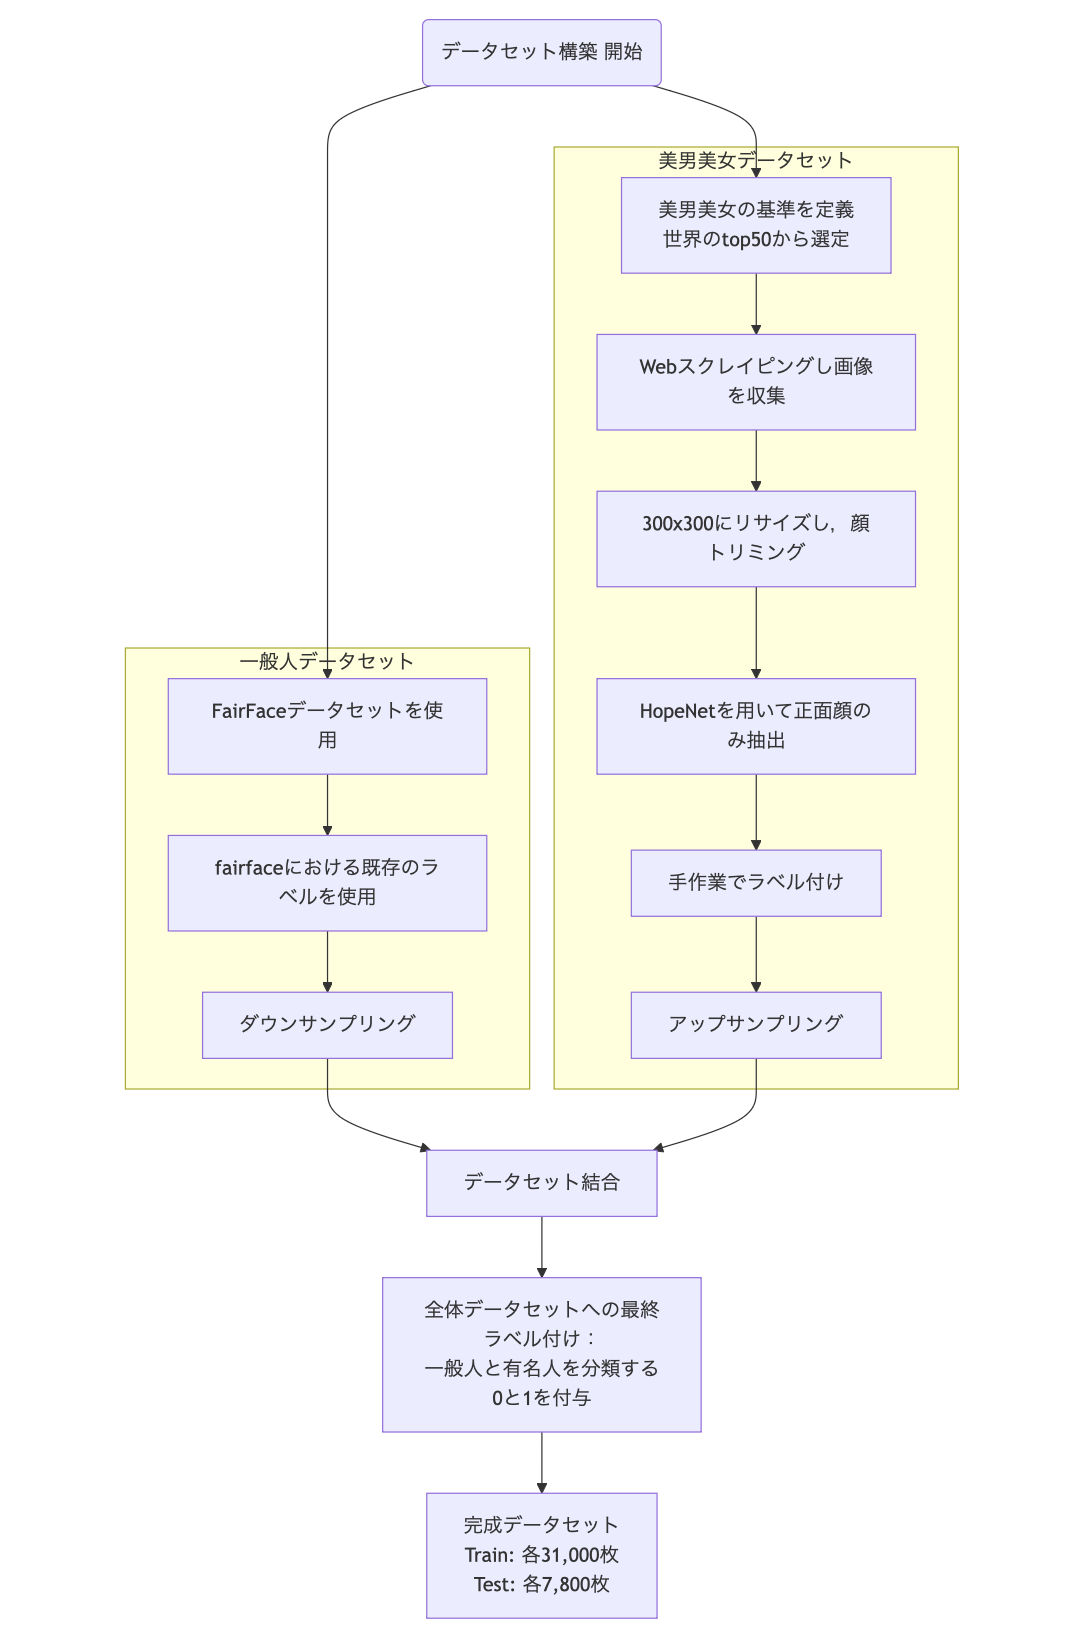
\includegraphics[width=0.9\textwidth]{final_rep_G1.png}
    \caption{前処理のフローチャート}
    \label{fig:csv}
\end{figure}
%======================


\subsection{モデル選定}
FairFaceが提供する学習済みモデルを本研究のタスクに合わせてカスタマイズした。これにはResNet34が使用されていたため,そのままResNet34を用いる。詳しくは\cite{karkkainenFairFace}を参照されたい。\par
(後述するが,このFairFaceのカスタマイズモデルは精度が100\%になったため,別アプローチとして本実験ではFairFaceを用いず新規にResNet18, ResNet34, ResNet50も用いた。パラメータ調整はデフォルトのままである。)



\subsection{パラメータ調整}
デフォルト値のまま使用している。
GitHubに公開されているコードでは,ハイパーパラメータが不明であるが,\cite{karkkainenFairFace}より学習率0.0001のOptimizerにADAM最適化が用いられている。これらのハイパーパラメータが選ばれた理由はGitHubや論文を読んでも不明である。
% 学習率は0.0001で、ADAM最適化を行っている。

\section{実験}

\subsection{役割分担について}
\begin{itemize}
    \item 215706D:KIM HYUNWOO
        \begin{itemize}
            \item 正面画像抽出・ラベル付・複数のResNetとEfficientNetでの実行・Grad Cam
        \end{itemize}
    \item 235221E:山脇大輝
        \begin{itemize}
            \item FairFaceの調査,カスタマイズ,Webスクレイピング・リサイズ・トリミング・ラベル付
        \end{itemize}
    \item 235701B:松田遼平
        \begin{itemize}
            \item GitHubの操作補助
        \end{itemize}
    \item 235732B:長\UTF{7028}一生
        \begin{itemize}
            \item アップサンプリング・ダウンサンプリングコード作・背景のマスキング実施
        \end{itemize}
\end{itemize}

%\subsection{実験設計}
%\begin{itemize}
%    \item 実験の目標
%    \item 目標をどのように達成しようとしたのか
%\end{itemize}


\subsection{用意したデータセット画像}
図\ref{fig:good_ex},図\ref{fig:normal_ex}に用意したデータセットの画像の一部を示す。これは筆者がランダムに選択したものであり,レポートの可読性を向上させるために用意した。
%======================
\begin{figure}[htbp]
    \centering
    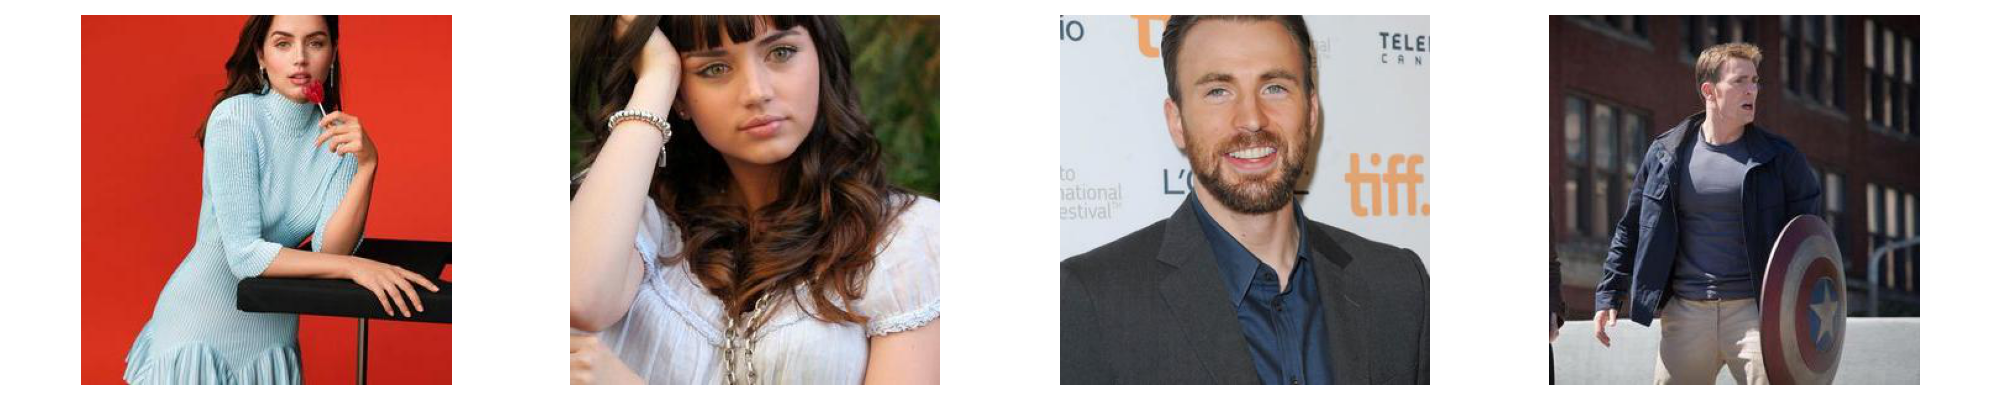
\includegraphics[width=1.1\textwidth]{ex_good_dataset.png}
    \caption{有名人データセットの画像例}
    \label{fig:good_ex}
\end{figure}
%======================
%======================
\begin{figure}[H]
    \centering
    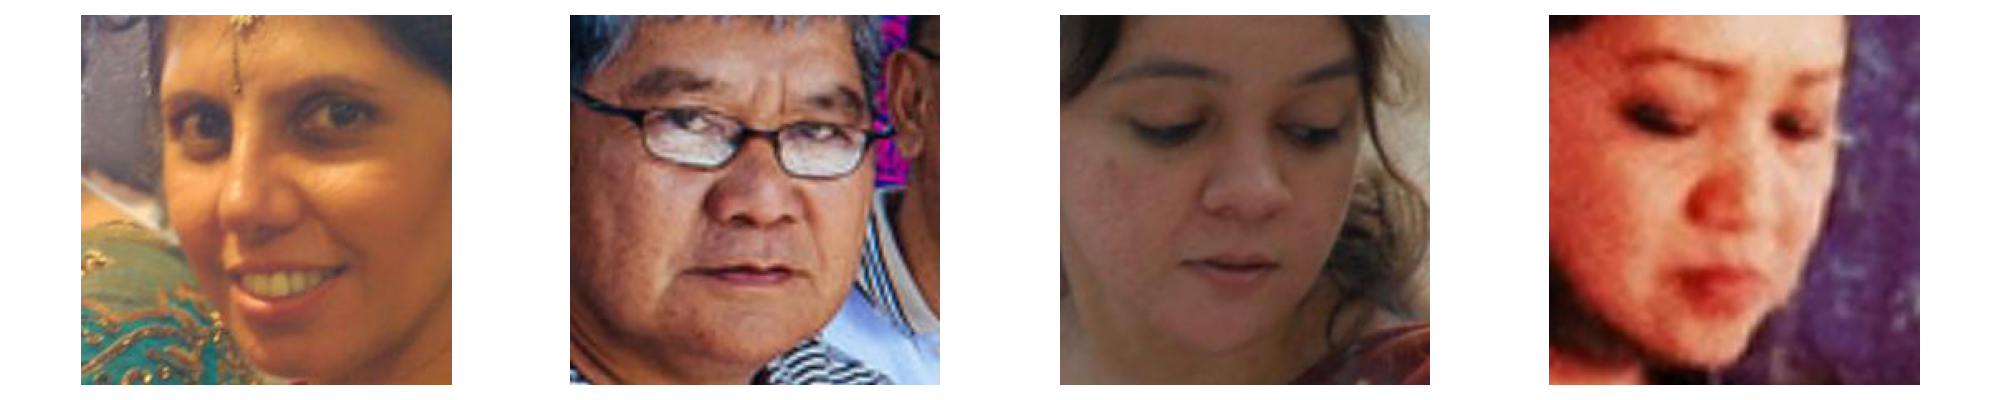
\includegraphics[width=1.1\textwidth]{ex_normal_dataset.png}
    \caption{一般人データセットの画像例}
    \label{fig:normal_ex}
\end{figure}
%======================


\section{実験結果}
FairFaceが提供する学習済みモデルを本研究のタスクに合わせてカスタマイズしたResNet34を用いた実行結果を表\ref{tab:custom}に示す。

\subsection{Custom Model}
\begin{table}[H]
\centering
\caption{Custom Model}
\label{tab:custom}
\begin{tabular}{lrr}
\hline
 Epoch &  Train Accuracy &  Validation Accuracy \\
\hline
     1 &           99.48 &               100.00 \\
     2 &          100.00 &                99.99 \\
     3 &          100.00 &                99.99 \\
     4 &           99.97 &               100.00 \\
     5 &          100.00 &               100.00 \\
     6 &          100.00 &               100.00 \\
     7 &          100.00 &               100.00 \\
     8 &          100.00 &               100.00 \\
     9 &          100.00 &               100.00 \\
    10 &          100.00 &               100.00 \\
\hline
\end{tabular}
\end{table}
% 原因:過学習(valで結果が出ているから問題ない。)・データのリーク(=> 原因としてわかんない)・追加学習だからわかんないよ。
% 

考察:
学習済みモデルであるFairFaceに追加学習を行ったCustom Modelは,エポック1からtrainの精度99.48\%,valの精度100.00\%と極めて高い精度を示した。エポック2以降もtrain,valの精度の共にほぼ100\%に達しており,過学習が発生している可能性が高い。また,どの部分を見て学習したのかは不明瞭かつ判断が困難である。

\subsection{Custom Modelの結果の透明性確保(仮説立て)}
本研究の目的はFairFaceに追加学習をすることによって有名人と一般人の差異を明らかにすることであった。しかし,FairFaceに追加学習したモデル(Custom Model)は精度が100\%になった。FairFaceはそもそも学習済みモデルであり,それに追加学習を行うアプローチのため,過学習の影響なのか,学習済みモデルや追加学習に起因したものなのか,原因の切り分けが困難である。\par
表\ref{tab:custom}から過学習による傾向は見られず,過学習をしているとは考えにくい。\\
では,なぜここまでの高精度が実現できているかを原因分析すると,以下の2点が挙げられる。
\begin{itemize}	
	\item \textbf{要因1.} FairFace の学習済みモデルが持つ広い表現能力(性別・人種・年齢分類)に対し,本タスク(有名人/一般人分類)が比較的容易な問題であったため,追加学習によって早期に分離境界を発見でき,このような高精度になった
	\item \textbf{要因2.} 画像の枚数の違い
	\begin{itemize}
		\item fairfaceでは\cite{karkkainenFairFace}より,108,501枚の学習データが使用されている。私たちが用意したデータセットの画像数は,およそtrain で31000 枚ずつ,test で7800 枚ずつであり,そもそも学習している画像の枚数に違いがあるのではないかと考えられる。
	\end{itemize}
	\item \textbf{要因3.} パラメータ調整の違い
	\begin{itemize}
		\item FairFaceのモデルが高精度を実現した原因として適切なパラメータ調整が考えられるが,\cite{karkkainenFairFace}やGitHub等を見ても与えられているのは学習済みモデルを使って予測するコードであり,具体的にどのようにパラメータ調整が行われたのかは不明である。
	\end{itemize}
	\item \textbf{要因4.} 構築したデータセットの問題
	\begin{itemize}
		\item 構築したデータセットは一般人のデータセットは新規で用意しておらず,FairFaceの学習済みモデルですでに使用された画像データをダウンサンプリングした上で再度有名人の画像群とともに学習させている。そのため一般人のデータを学習時に背景を見る傾向にある可能性がある。
	\end{itemize}
\end{itemize}
% we constructed a novel face image dataset containing 108,501 images which is balanced on Race.  

追加学習を行って100\%の精度を達成したが,この精度の妥当性を検証する。
上記仮説に基づき,違うアプローチとして,新規に学習を行い,それらと追加学習を行ったものを比較し,精度や追加学習を行ったため元のFairFaceの性別・人種・年齢分類と比べて有名人・一般人の二値分類タスクが簡単だったのかを確かめる。
ここで,新規学習で用意したモデルはResNet18,ResNet34,ResNet50とEfficientNet\_b0であり,これらはCustom Modelと同じパラメータ調整を行った。


\section{仮説検証1:新規学習}
ResNet18,ResNet34,ResNet50とEfficientNetのモデルで新規学習を行なった実行結果を表\ref{tab:ResNet18},表\ref{tab:ResNet34},表\ref{tab:ResNet50},表\ref{tab:efficientnet}に示す。

\subsection{ResNet 18}
\begin{table}[H]
\centering
\caption{ResNet-18}
\label{tab:ResNet18}
\begin{tabular}{lrr}
\hline
 Epoch &  Train Accuracy &  Validation Accuracy \\
\hline
     1 &           97.92 &                99.28 \\
     2 &           99.23 &                99.22 \\
     3 &           99.47 &                99.53 \\
     4 &           99.61 &                99.48 \\
     5 &           99.68 &                99.52 \\
     6 &           99.76 &                99.38 \\
     7 &           99.83 &                99.59 \\
     8 &           99.83 &                99.51 \\
     9 &           99.88 &                99.45 \\
    10 &           99.88 &                99.52 \\
\hline
\end{tabular}
\end{table}

考察:ResNet-18は,trainの精度97.92\%から99.88\%まで順調に向上した一方,valの精度は99.2\%から99.6\%の範囲で安定して推移していることがわかる。trainとvalの値が激しく乖離しておらず,適切に学習できているだろうと結論づけられる。


\subsection{ResNet 34}
\begin{table}[h]
\centering
\caption{ResNet-34}
\label{tab:ResNet34}
\begin{tabular}{lrr}
\hline
 Epoch &  Train Accuracy &  Validation Accuracy \\
\hline
     1 &           97.74 &                99.08 \\
     2 &           99.27 &                99.34 \\
     3 &           99.40 &                99.27 \\
     4 &           99.55 &                99.50 \\
     5 &           99.59 &                99.40 \\
     6 &           99.65 &                99.27 \\
     7 &           99.72 &                99.31 \\
     8 &           99.80 &                99.49 \\
     9 &           99.79 &                99.56 \\
    10 &           99.84 &                99.47 \\
\hline
\end{tabular}
\end{table}

考察:ResNet-34の結果は,ResNet-18と同様の傾向を示している。前述のResNet18よりも層が深くなっているものの,検証の精度自体に著しい向上が見られなかったことから,ResNet18の時点で十分にモデルの表現能力が達成されており,これ以上層を増やしてもこれ以上の性能向上は見込めないだろう。

\subsection{ResNet 50}

\begin{table}[H]
\centering
\caption{ResNet-50}
\label{tab:ResNet50}
\begin{tabular}{lrr}
\hline
 Epoch &  Train Accuracy &  Validation Accuracy \\
\hline
     1 &           95.26 &                98.58 \\
     2 &           98.69 &                98.76 \\
     3 &           99.10 &                99.20 \\
     4 &           99.32 &                99.25 \\
     5 &           99.39 &                99.34 \\
     6 &           99.50 &                99.37 \\
     7 &           99.54 &                99.40 \\
     8 &           99.66 &                99.28 \\
     9 &           99.71 &                99.36 \\
    10 &           99.75 &                99.39 \\
\hline
\end{tabular}
\end{table}

考察:ResNet-18やResNet-34の性能を上回ることはなく,ResNetでは層を深くしても(18→34→50)顕著な性能向上は見られなかった。さらには訓練初期の精度が他のResNetモデルより低い(95.26\%)ことから,モデルの複雑性が増した分学習の収束に時間を要する可能性が考えられる。本データセットの分類タスクの複雑性に対して、ResNet-18の時点ですでにモデルの表現力が十分であったことが考えられる。
%モデルの層を増やすよりかはパラメータ調整の方が有益であろう。


\subsection{EfficientNet}

\begin{table}[H]
\centering
\caption{EfficientNet}
\label{tab:efficientnet}
\begin{tabular}{lrr}
\hline
 Epoch &  Train Accuracy &  Validation Accuracy \\
\hline
     1 &           94.47 &                98.76 \\
     2 &           99.00 &                99.19 \\
     3 &           99.40 &                99.54 \\
     4 &           99.63 &                99.59 \\
     5 &           99.79 &                99.79 \\
     6 &           99.85 &                99.82 \\
     7 &           99.89 &                99.94 \\
     8 &           99.92 &                99.96 \\
     9 &           99.93 &                99.87 \\
    10 &           99.95 &                99.96 \\
\hline
\end{tabular}
\end{table}


考察:train,valの精度の両方がエポックの進行と共に安定して向上し,最終的にはエポック10で99.86という高い値を更新している。
\subsection{Custom Modelと新規学習の比較}

新規学習のモデルは,Custom Modelと比較しても高精度で実現できており,この新規学習のアプローチでは仮説検証を行えなかった。そこで正しく顔のみを見て分類し,ここまで高い精度を実現できているかは不透明であるため,Grad-Camによる検証も行う。


\section{仮説検証2:Grad-Camを用いたモデルの信頼性の検証}
\subsection{検証の概要}
Grad-CAM(Gradient-weighted Class Activation Mapping)というCNNが画像のどの部分に注目して一般人か美男美女かの判断を下したのかをヒートマップとして可視化する技術がある。
図\ref{fig:gradcam_good},図\ref{fig:gradcam_normal}にGrad-CAMを用いてモデルごとに有名人(good)と一般人(normal)の各データの平均したヒートマップを示す。
本研究で得られた99\%超という検証精度の原因を探る。
各画像は以下に示すモデルを適用した結果である。
\begin{itemize}
	\item 1行目
	\begin{itemize}
	\item 追加学習したモデル:custom
	\item EfficientNet\_b0
	\item ResNet18
	\end{itemize}
	\item 2行目
	\begin{itemize}
	\item ResNet34
	\item ResNet50
	\end{itemize}
\end{itemize}


\subsection{検証結果}
%======================
\begin{figure}[H]
    \centering
    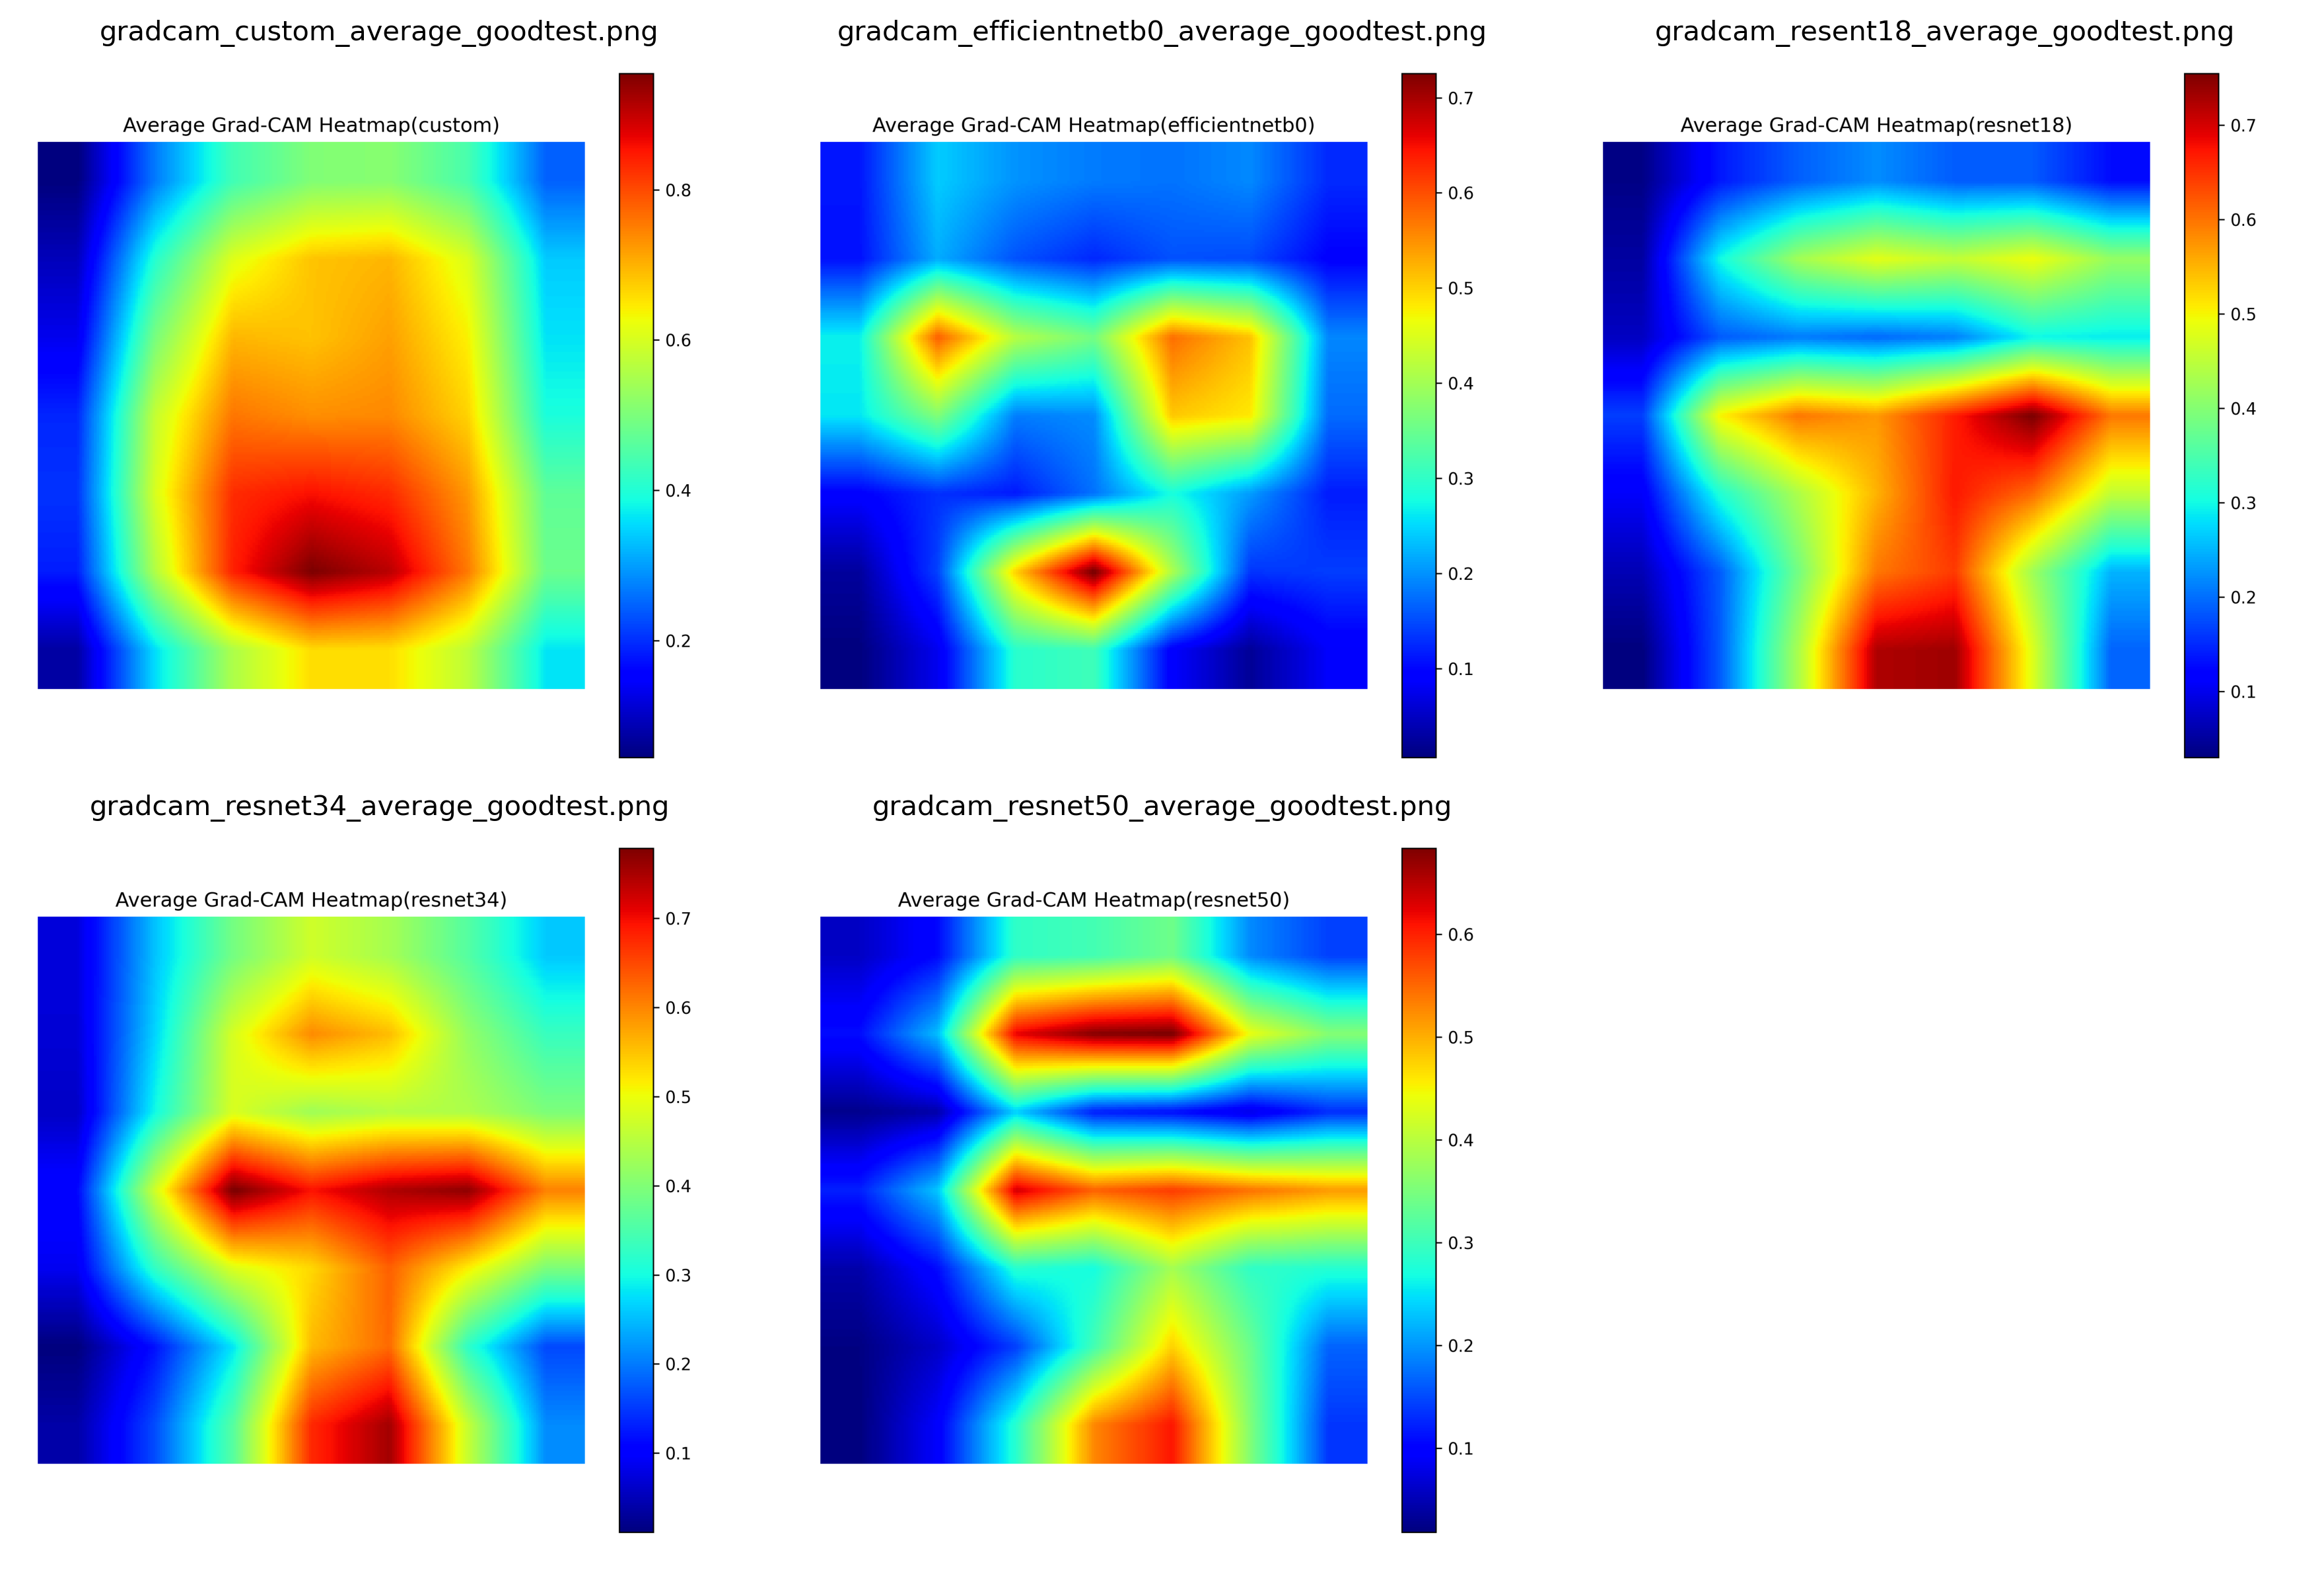
\includegraphics[width=1.1\textwidth]{combined_images_good.png}
    \caption{Grad-CAMを用いた有名人の判断根拠の可視化}
    \label{fig:gradcam_good}
\end{figure}
%======================
%======================
\begin{figure}[H]
    \centering
    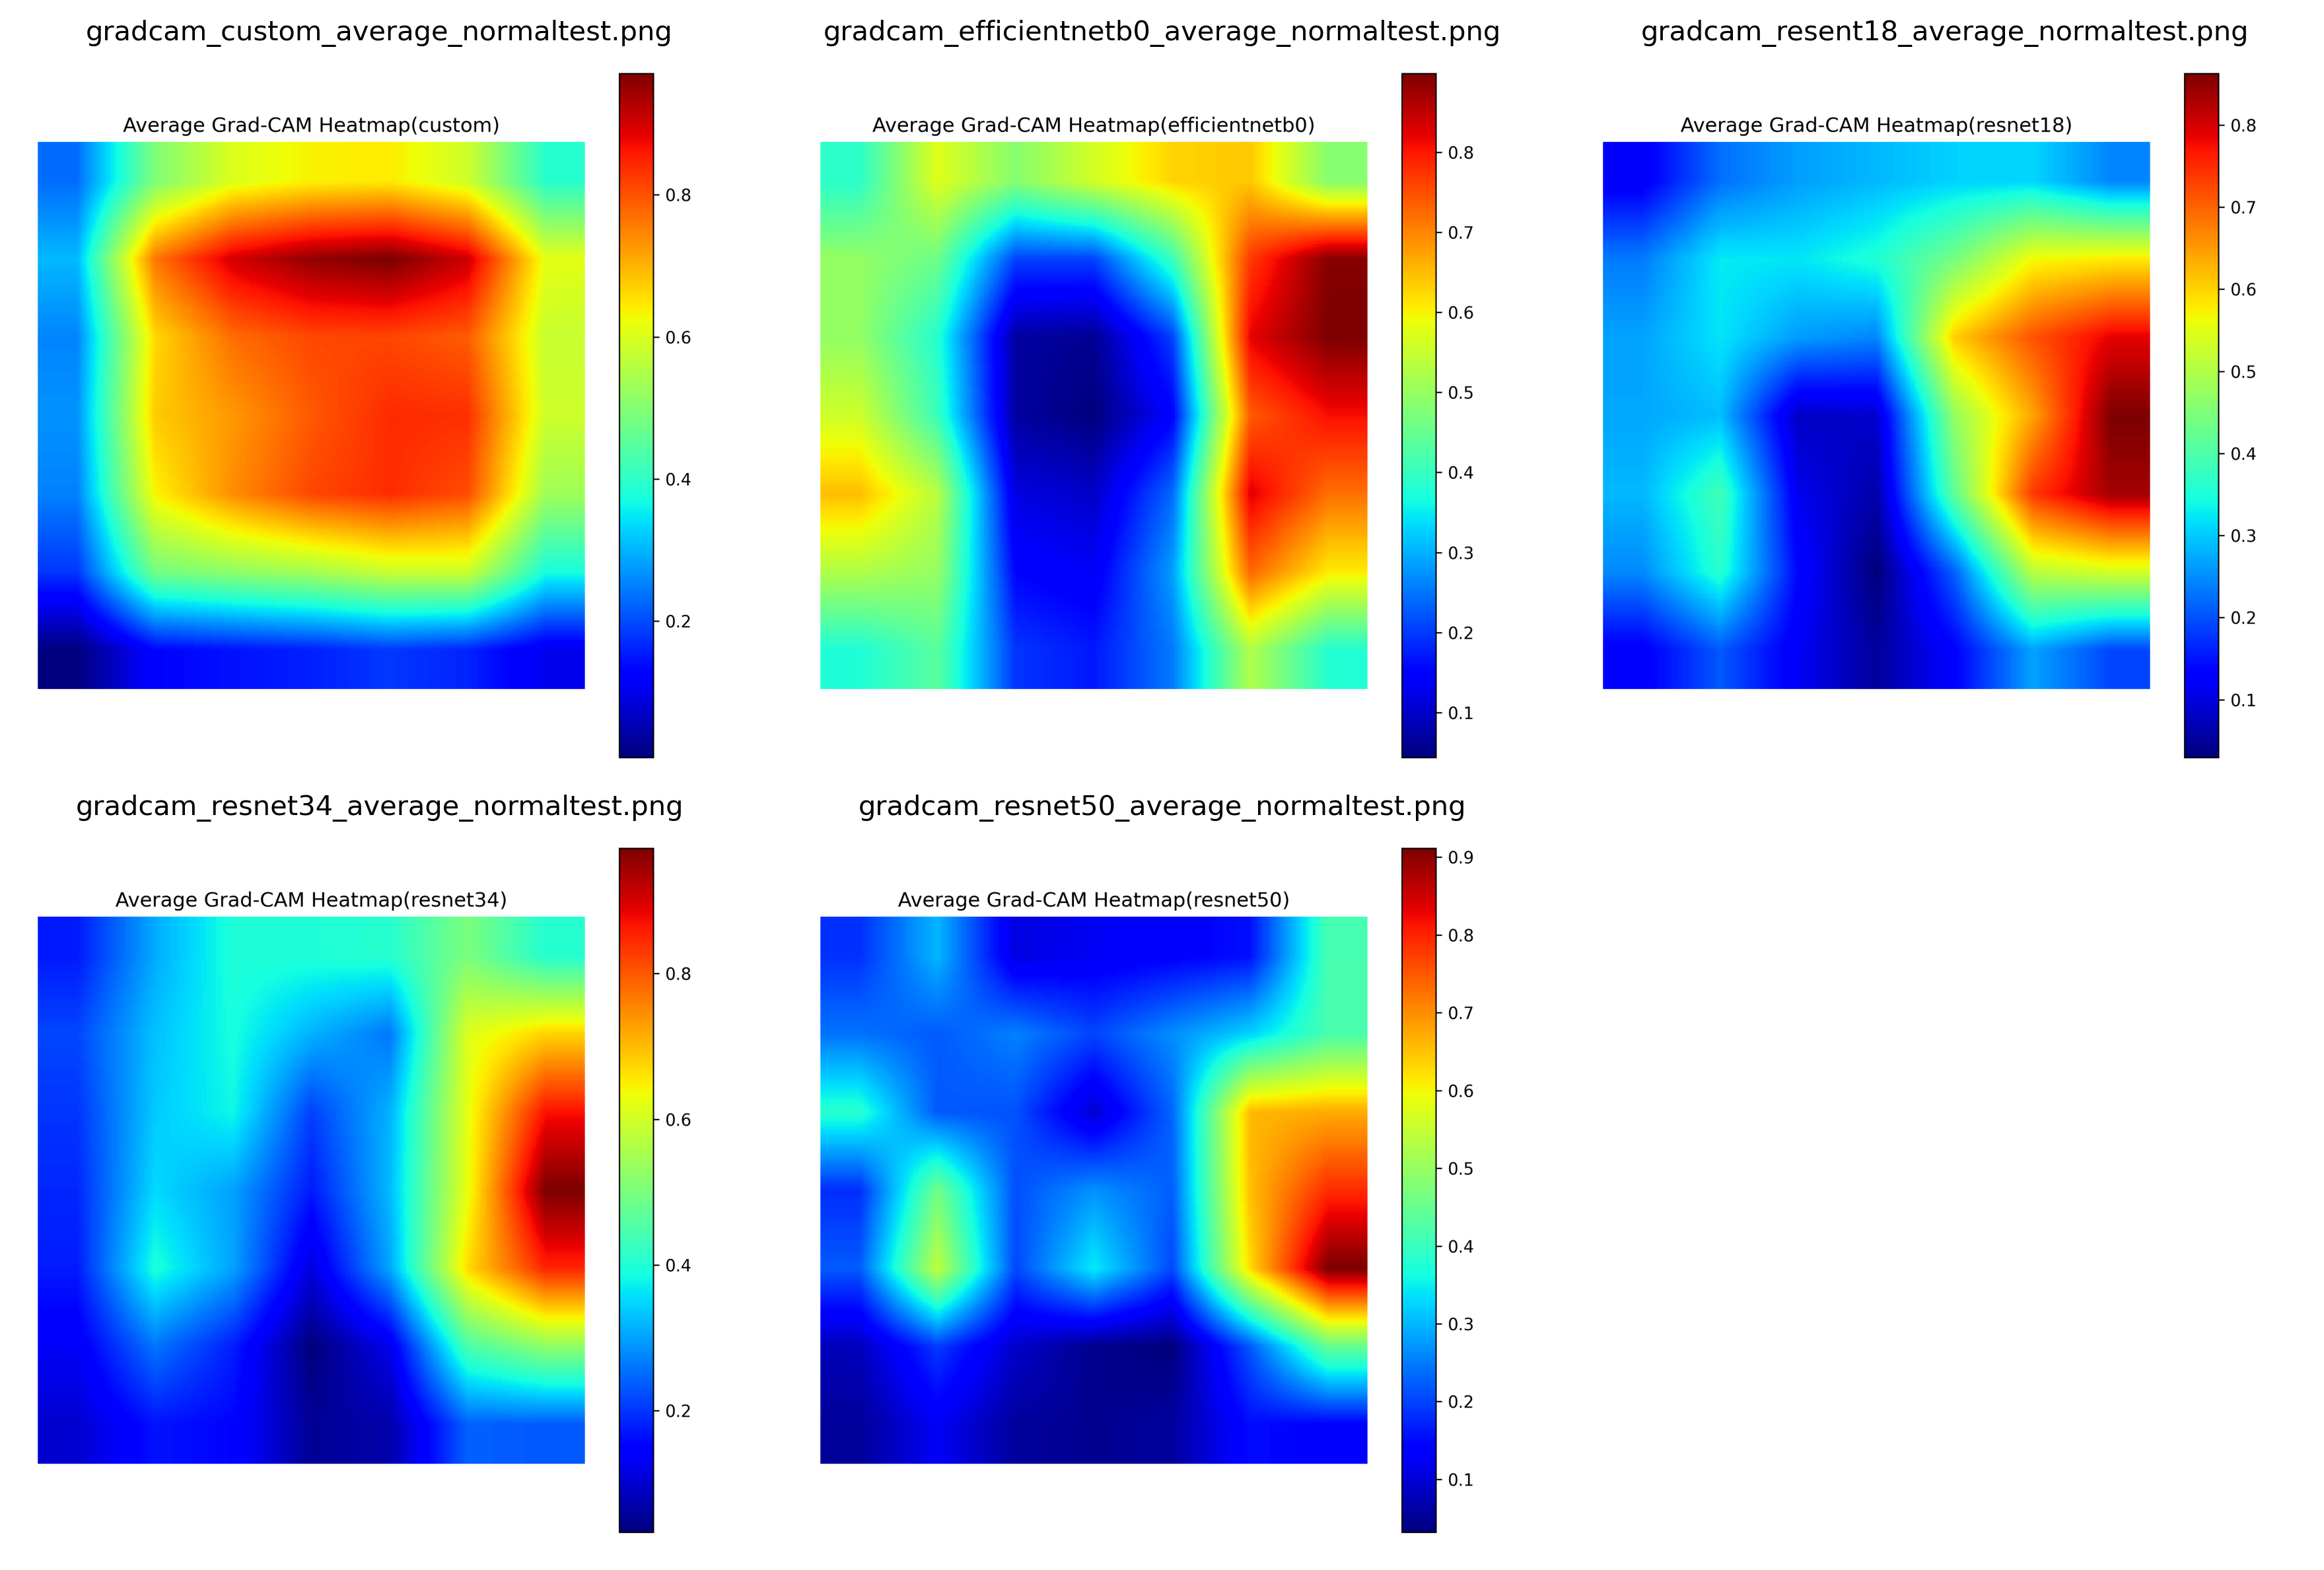
\includegraphics[width=1.1\textwidth]{combined_images_normal.png}
    \caption{Grad-CAMを用いた一般人の判断根拠の可視化}
    \label{fig:gradcam_normal}
\end{figure}
%======================

\subsubsection{検証結果の考察}
有名人の判断根拠について,customeは顔全体,特に口元がよく見られているが,それ以外のResNet・EfficientNetについては,全体の傾向として,目と口が判断根拠になっていることがわかる。\par
一方,一般人の判断根拠について,customモデルは目元の上部(額と思われる)を見ており,それ以外のモデルは人物の右背景を見ていることがわかる。右背景を見ているのでは目的であった顔を見て分類する目的を果たせておらず,実験の目標は達成できていない。そこで次の章では,これらの背景の影響を抑えるために画像を白背景にして再度を学習を行った。
%ただし,用意したデータセットをモデルごとに実行し,Grad-Camで得た出力の「モデルごとの平均」であることに注意したい。




\subsection{白背景画像を用いたGrad-Camの改善}
\subsubsection{検証の概要}

背景情報への依存を低減させる試みとして全画像の背景を白色に加工し,再度学習を行なった。
図\ref{fig:gradcam_good_white},図\ref{fig:gradcam_normal_white}にGrad-CAMを用いてモデルごとに有名人(good)と一般人(normal)の各データの平均したヒートマップを示す。

各画像は以下に示すモデルを適用した結果である。
\begin{itemize}
	\item 1行目
	\begin{itemize}
	\item 追加学習したモデル:custom
	\item EfficientNet\_b0
	\item ResNet18
	\end{itemize}
	\item 2行目
	\begin{itemize}
	\item ResNet34
	\item ResNet50
	\end{itemize}
\end{itemize}


\subsubsection{検証結果}
%======================
\begin{figure}[H]
    \centering
    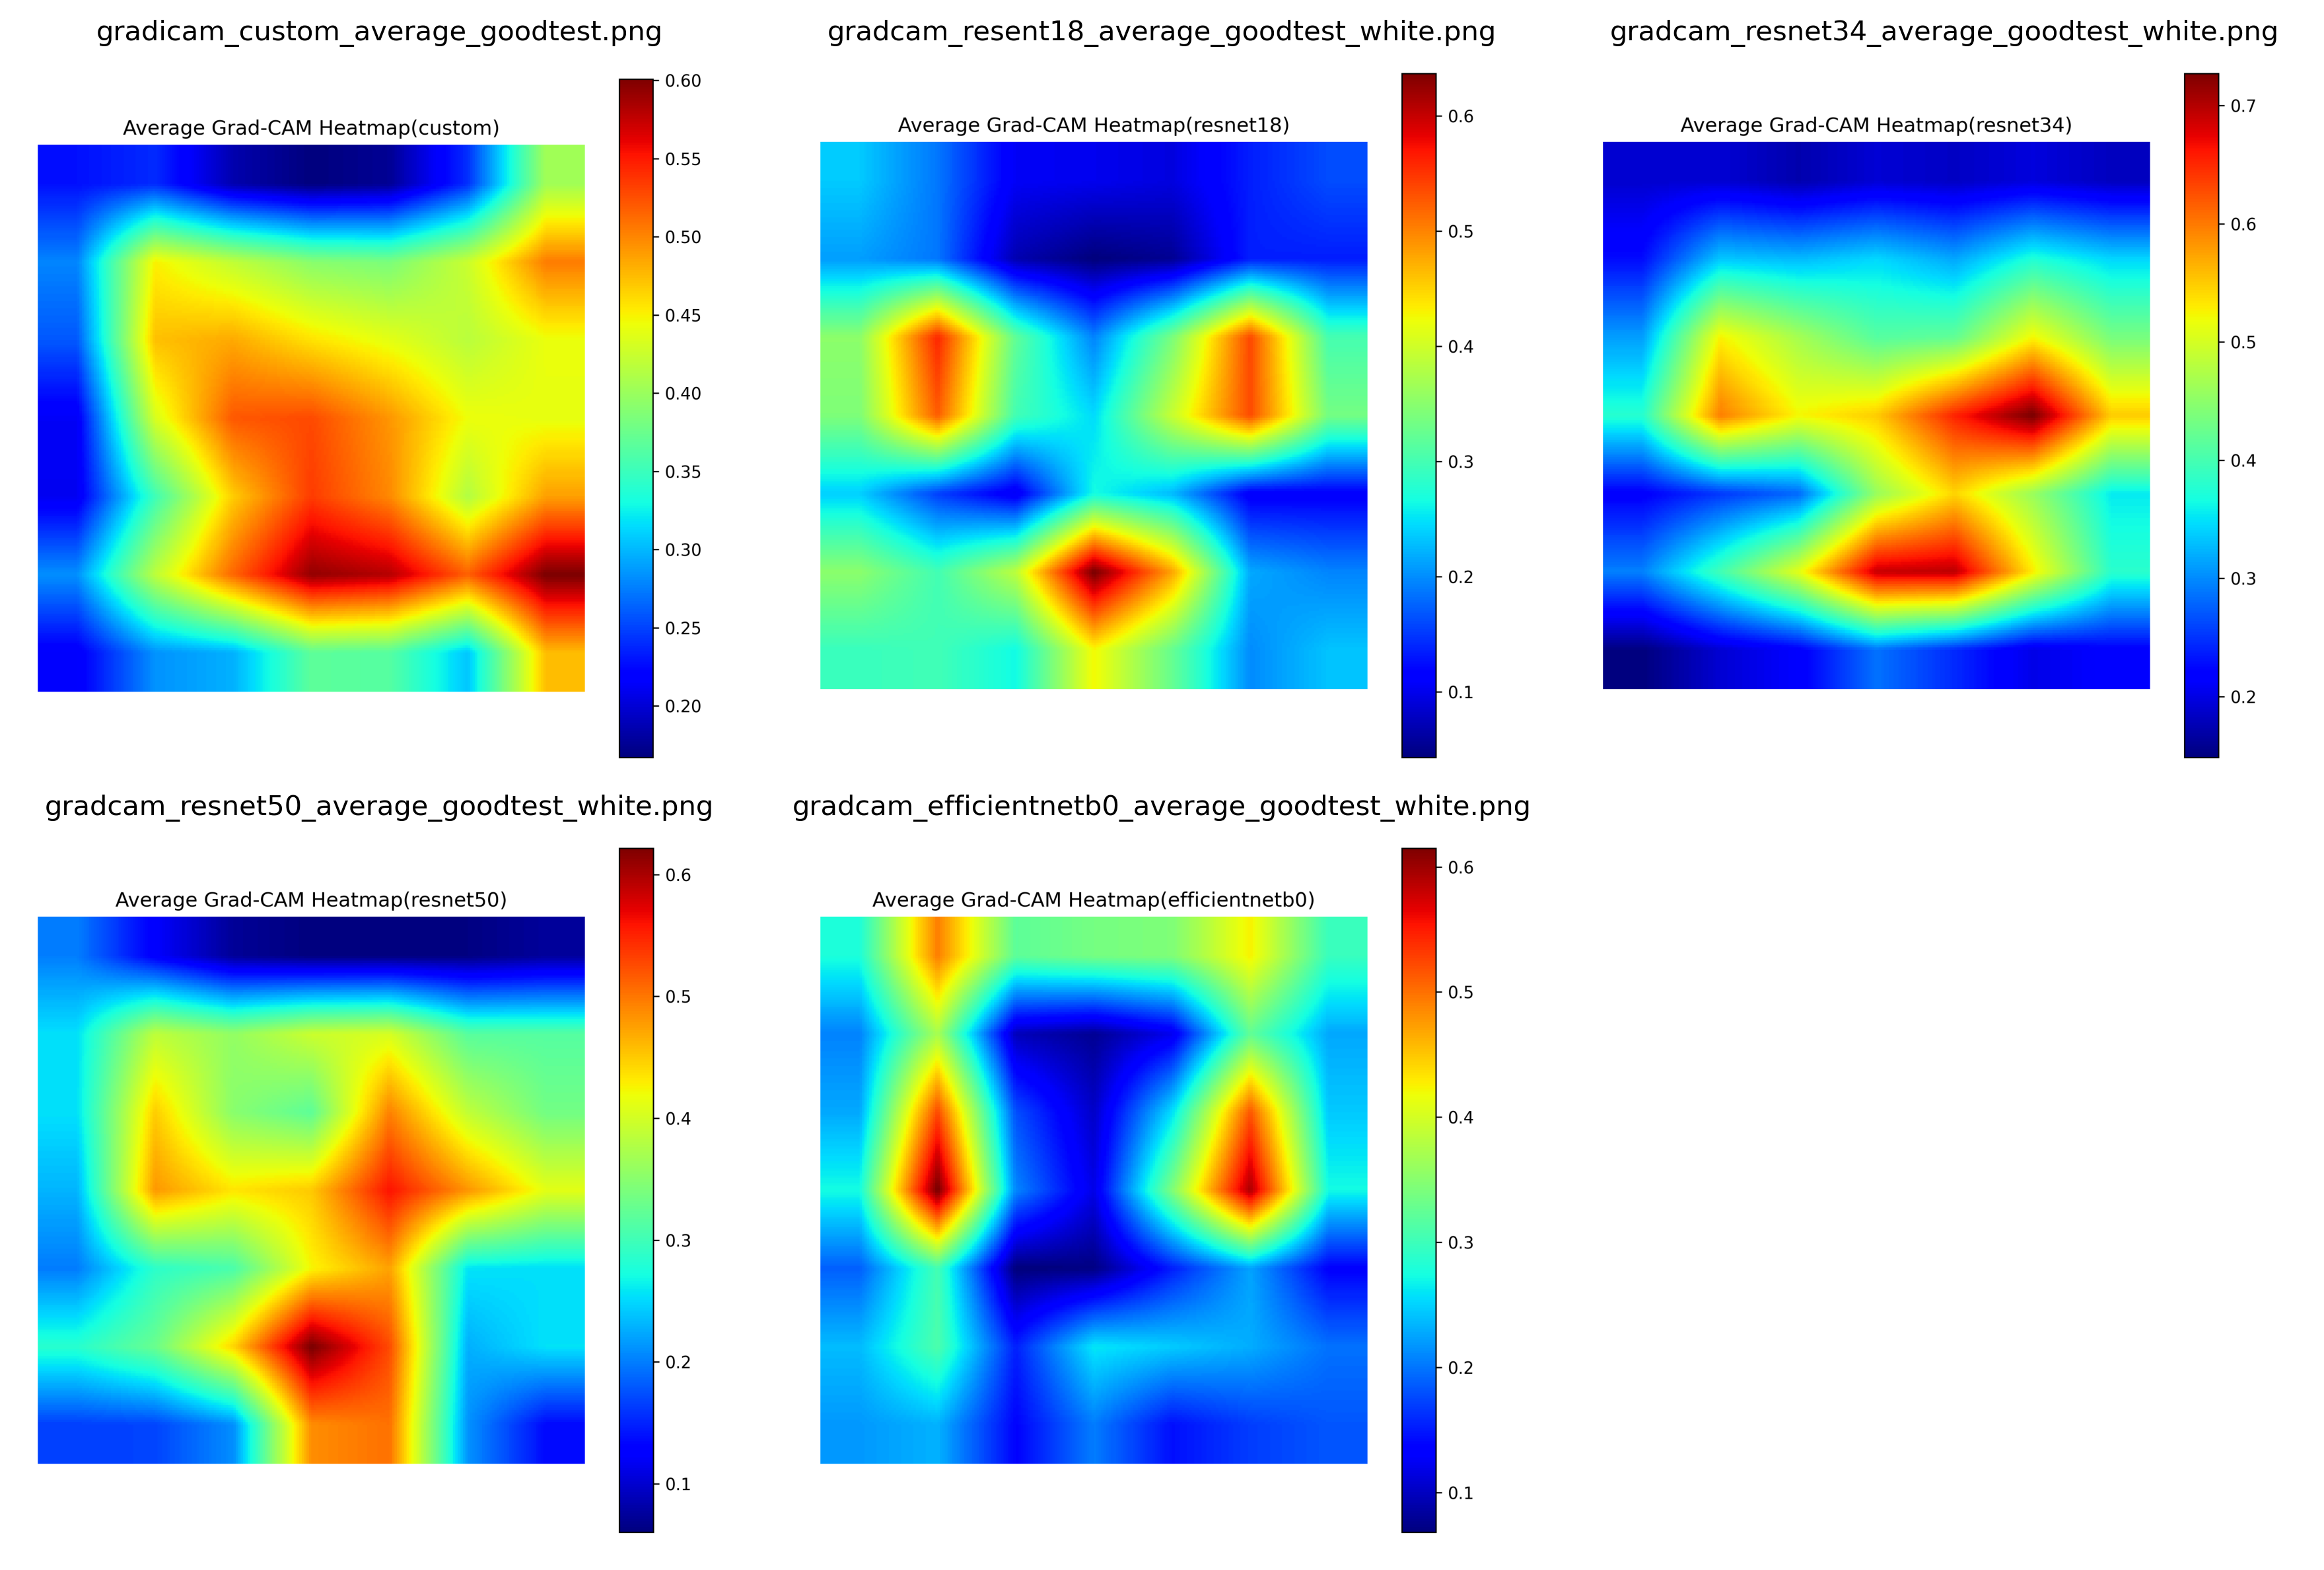
\includegraphics[width=1.1\textwidth]{white_combined_images_good.png}
    \caption{白背景でのGrad-CAMを用いた有名人の判断根拠の可視化}
    \label{fig:gradcam_good_white}
\end{figure}
%======================
%======================
\begin{figure}[H]
    \centering
    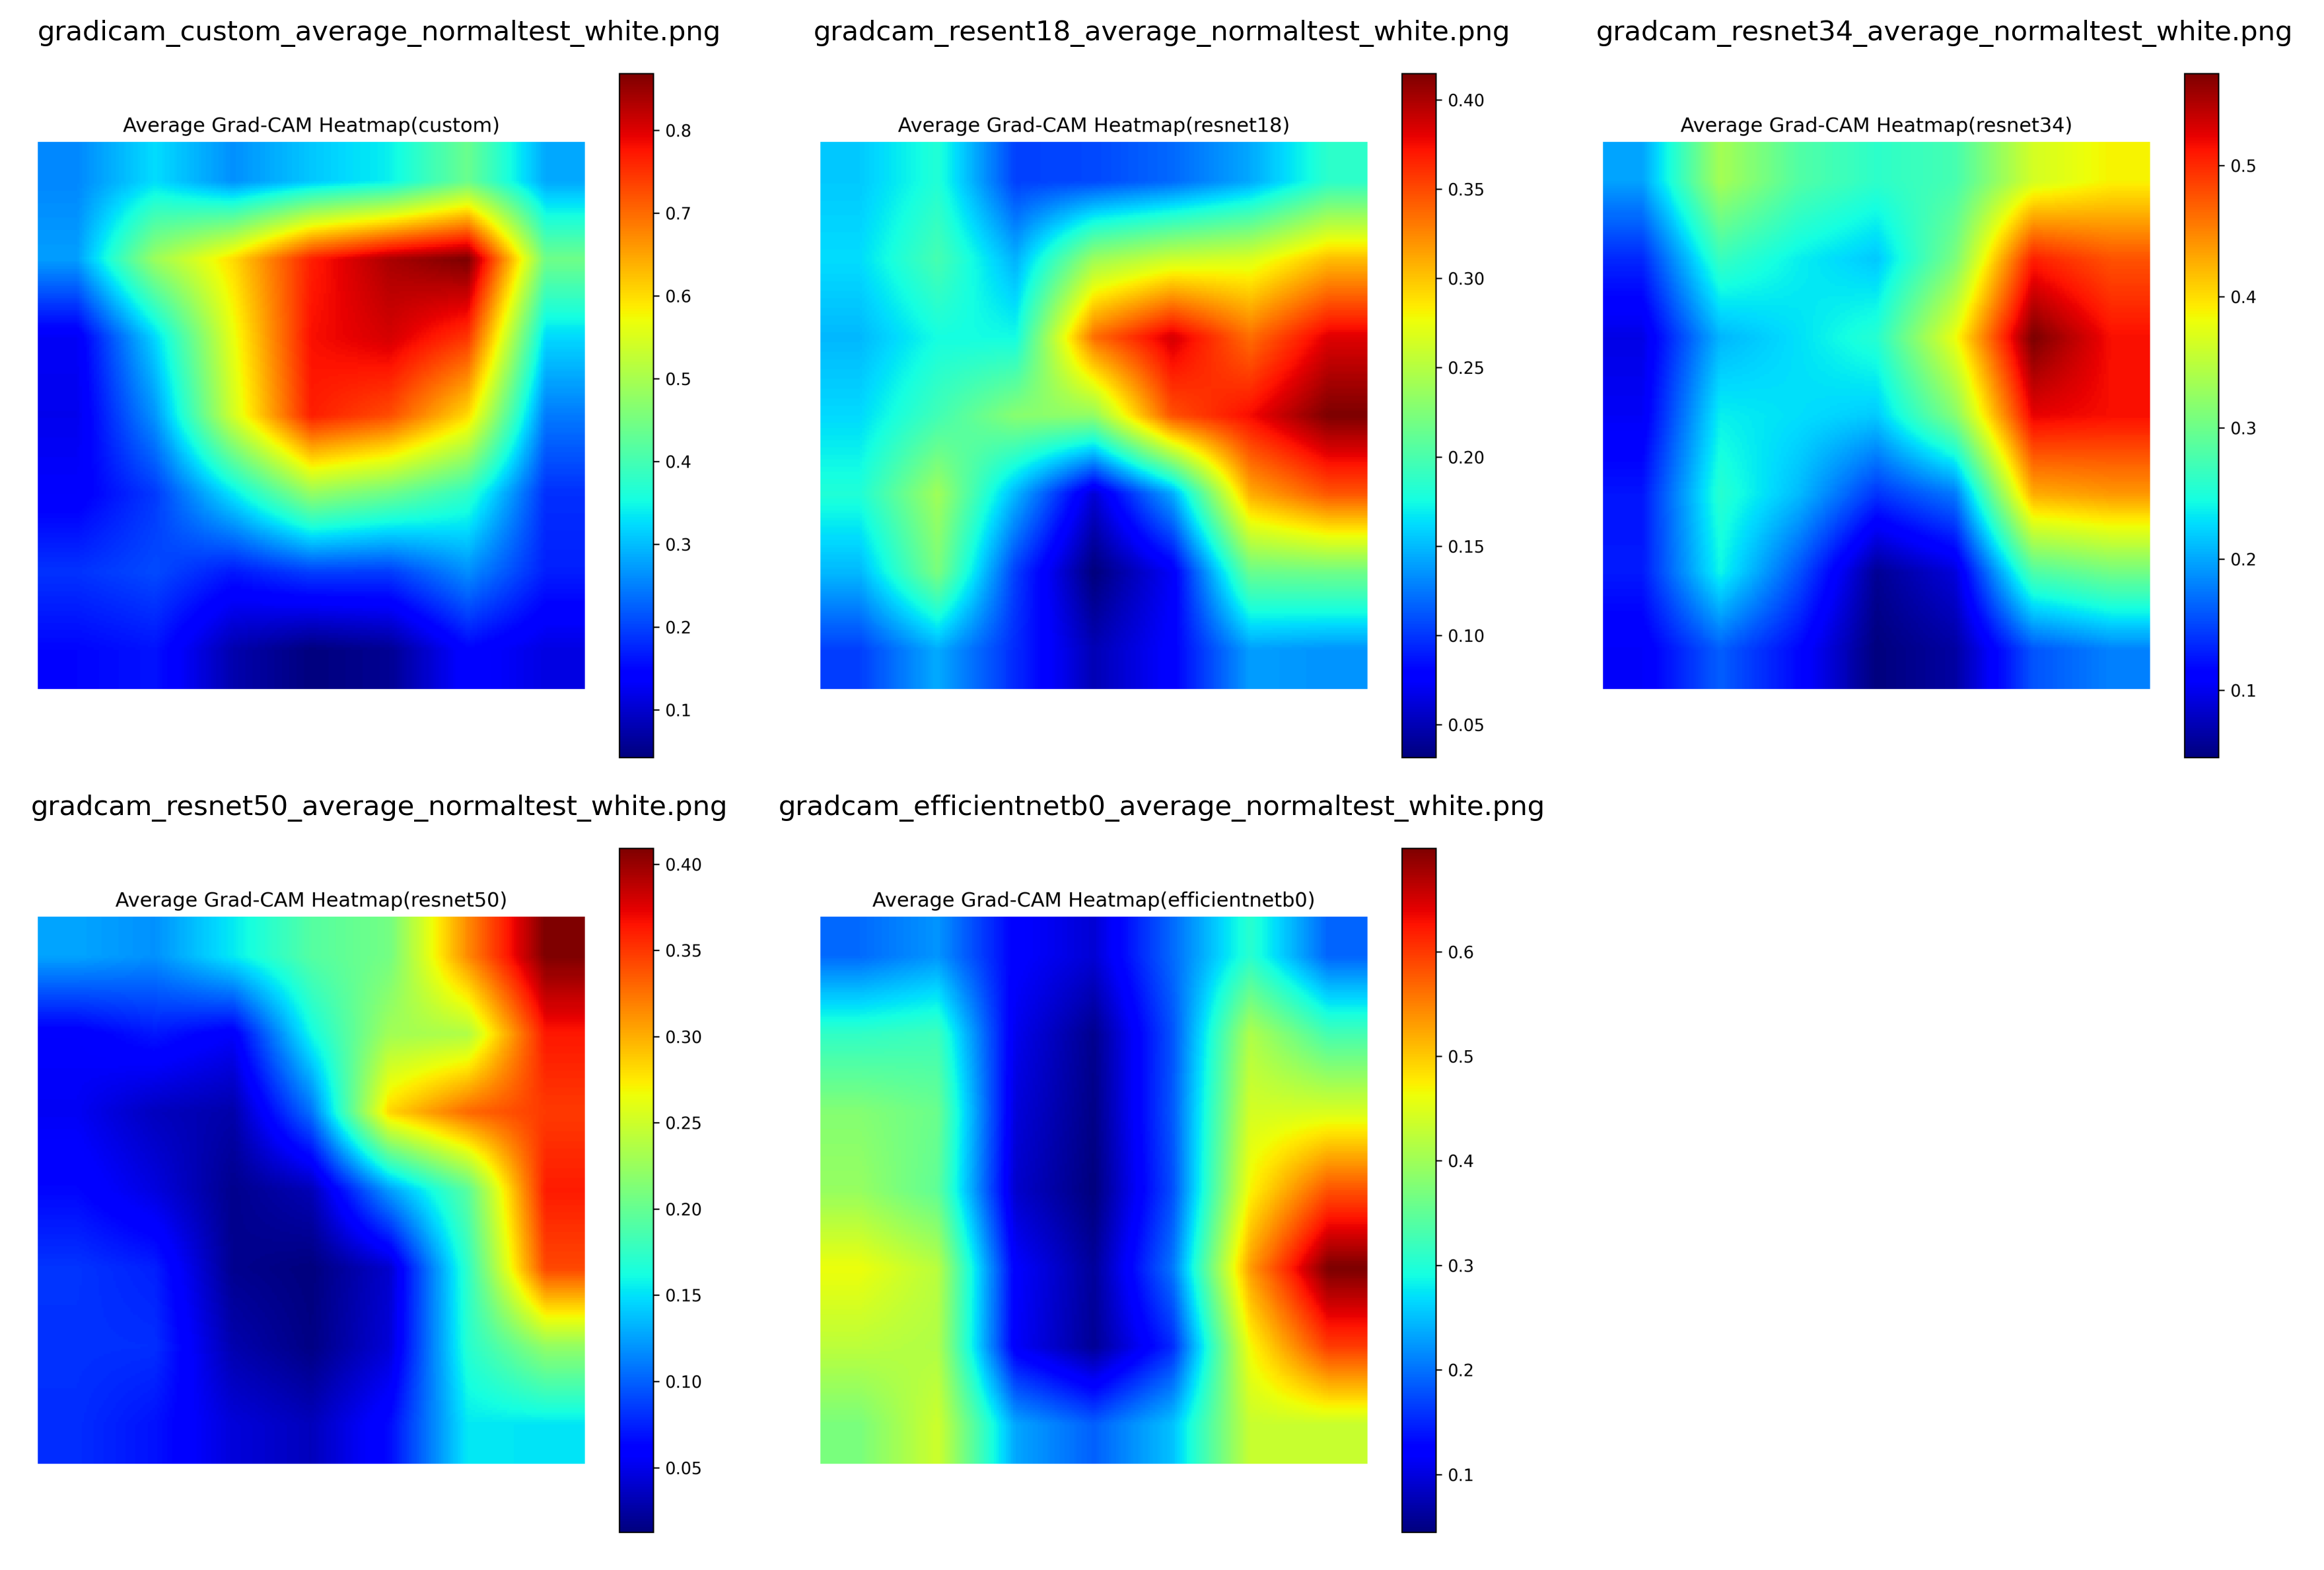
\includegraphics[width=1.1\textwidth]{white_combined_images_normal.png}
    \caption{白背景でのGrad-CAMを用いた一般人の判断根拠の可視化}
    \label{fig:gradcam_normal_white}
\end{figure}
%======================


\subsection{検証結果・考察}

有名人の判断根拠については,先ほどと同様に顔全体,特に目元・口元がよく見られているが,EfficientNetについては,顔から離れた背景ないしは目元を注視している。\par
しかしながら,一般人の判断根拠については白背景の有無に関わらず右背景を見ている傾向にある。

一方,一般人の判断根拠について,右背景を注視する傾向にあり,人物には注目できていないことがわかる。
%ただし,用意したデータセットをモデルごとに実行し,Grad-Camで得た出力の「モデルごとの平均」であることに注意したい。


この原因については,図\ref{fig:good_ex},図\ref{fig:normal_ex}に示したように有名人の画像の全体的な傾向として,記者会見などで用いられるバックパネルやスタジオで撮影されていると思われる画像など,背景がシンプルなものが多い。また人物の写りがよくなるように画像加工されていたり,有名人の写真はいわゆる一眼レフなどの良いカメラが使われていたりといった可能性も考えられる。

一方で,一般人の画像は,Flickr 画像とTwitterやオンライン新聞の画像などがデータセットに使われており,人物の横に他の人の体の一部が写っているなどの背景が乱雑なものやカメラを向いていなかったりするものが多い傾向にある。そういった構築したデータセットの画像の特徴から,一般人の分類において背景で判断されたと考えられる。\\


しかし,それを踏まえたとしてもCustom Modelは正しく顔を捉えることができており,前述した仮説による影響が考えられる。したがって,検証結果よりCustom Modelの精度が高い理由は


\section{まとめ}
%新規学習モデル群も非常に高い精度を達成したが、ResNetアーキテクチャでは層を深くしても(18→34→50)顕著な性能向上は見られなかった。これは、本データセットの分類タスクの複雑性に対して、ResNet-18の時点ですでにモデルの表現力が十分であったことが考えられる。
%新規学習モデルは分類時に特に画像の背景に依存している傾向にあり,これは構築したデータセットに含まれるバイアスの影響が大きい。


gradcamの実行結果を見ると,口と目が有名人と一般人で異なることが示唆される。





\section{反省・今後の課題}



githubを使おうとしたが,使える人数が少なくgithubでのバージョン管理が実質できていなかった。さらにamaneで実行する場合,さらにソースコードのバージョンが不透明になってしまった。
役割分担・実験計画が適切にできておらず,実験の後半で急いで学習を行った。計画よりも前処理に時間がかかり,その後も実行しその結果を考察する時間をファイルの欠損の対応・コンテナプラットフォームSingularity使用のための準備といった対応に終われてしまった。

\subsection{時間の都合上省いた項目}
\subsubsection{撮影日時による人物データの抽出}
画像をwebスクレイピングで収集したものについて,ネットに存在する有名人の画像は撮影された日時がバラバラである。若い時の写真もあれば現在の写真もあり,年齢によって発生する特徴量の変化については考慮できていない。検索キーワードをもとにスクレイピングをする際に,人名に年齢を含むアプローチも行ったが,得られる画像が少ない・検索してもそもそも年齢で絞れないという問題が発生した。本実験で調べる限りは実験の限界と判断し,他の前処理を丁寧に行う方を優先した。

\subsubsection{構築したデータセットの人名の偏り改善}
本実験では,2024年美男美女ランキングtop50をもとに,50名ずつ抽出し,アップサンプリング(左右反転)を施した。これは一般人のデータセットと比較して,偏りが生じる。他のアップサンプリングの方法として回転・輝度変更といった手法があるが,これらでさらにデータを増やすよりかは,美男美女の人名数を50名ずつよりさらに増やす方がバイアスを削減できると考える。本実験では時間の都合・第一回の実験時の計画がずれていたため省略した。

\section{まとめ}


\begin{thebibliography}{9}
    \bibitem{karkkainenFairFace}
    Karkkainen, Kimmo and Joo, Jungseock.
    FairFace: Face Attribute Dataset for Balanced Race, Gender, and Age for Bias Measurement and Mitigation.
    In \textit{Proceedings of the IEEE/CVF Winter Conference on Applications of Computer Vision}, pages 1548--1558, 2021.\\
        \url{https://arxiv.org/abs/1908.04913}
    
    \bibitem{bidanshi}
    Most Handsome Man In The World 2024, shiningawards.com, \\
    \url{https://shiningawards.com/most-handsome-man-in-the-world-2024/}
    
    \bibitem{bijoshi}
    Most Beautiful Faces 2024, gigazine.net, \\ \url{https://gigazine.net/gsc_news/en/20241229-most-beautiful-faces-2024/}
    
        \bibitem{hopenet_paper}
        Nataniel Ruiz Eunji Chong and James M. Rehg (Georgia Institute of Technology).
        Fine-Grained Head Pose Estimation Without Keypoints
         In \textit{The IEEE Conference on Computer Vision and Pattern Recognition (CVPR) Workshops}, pages 2074--2083, 2018. \\
          \url{https://arxiv.org/abs/1710.00925}

    \bibitem{hopenet}
    Head Pose Estimation, \url{https://github.com/natanielruiz/deep-head-pose}
    \bibitem{gradcam}Grad-CAM: Visual Explanations from Deep Networks via Gradient-based Localization, 
    Ramprasaath R. Selvaraju, Michael Cogswell, Abhishek Das, Ramakrishna Vedantam, Devi Parikh, Dhruv Batra,\\
    \url{https://arxiv.org/abs/1610.02391}
    
  %github repo: https://github.com/jacobgil/pytorch-grad-cam
\end{thebibliography}

\end{document}
